\documentclass{article}
\usepackage{amsmath}
\usepackage[german]{babel}

%\usepackage{plantuml}
\usepackage{tikz}
\usepackage{graphicx}


\title{Beleg UDP-Dateitransfer für Rechnernetze/Kommunikationssysteme}
\author{Tilman Ischner}
\date{\today}


\begin{document}
    \maketitle
    \newpage
    \tableofcontents



    \section{Aufgabenstellung}
    Erstellen Sie ein Programm (client + server) zur Übertragung beliebiger Dateien zwischen zwei Rechnern, basierend auf dem UDP-Protokoll. Das Programm soll mit der Sprache JAVA erstellt werden und im Labor S311 unter Linux lauffähig sein und dort vorgeführt werden. Folgende Punkte sind umzusetzen:
    \begin{itemize}
        \item Aufruf des Clients (Quelle) auf der Konsole mit den Parametern: Zieladresse (IP oder Hostname) + Portnummer + Dateiname + Protokoll (sw|gbn) (Bsp.: filetransfer client is311p1 3333 test.gif gbn)
        \item Aufruf des Servers (Ziel) mit den Parametern: Portnummer (Bsp.: filetransfer server 3333). Um die Aufrufe für Client und Server so zu realisieren ist ein kleines Bash-script notwendig (z.B.: java Clientklasse \$1 \$2 \$3)

        \item Auf dem Zielrechner (Server) ist die Datei unter Verwendung des korrekten Dateinamens im Pfad des Servers abzuspeichern. Ist die Datei bereits vorhanden, soll an den Basisnamen der neuen Datei das Zeichen „1“ angehängt werden. Client und Server sollten auch auf dem selben Rechner im selben Pfad funktionieren.
        \item Messen Sie bei der Übertragung die Datenrate und zeigen Sie am Client periodisch (z.B. jede Sekunde) den aktuellen Wert und am Ende den Gesamtwert an. Sie können sich bei der Anzeige am Konsolenprogramm wget orientieren.
        \item Implementieren Sie exakt das im Dokument Beleg-Protokoll vorgegebene Übertragungsprotokoll. Damit soll gewährleistet werden, dass Ihr Programm auch mit einem beliebigen anderen Programm funktioniert, welches dieses Protokoll implementiert.
        \item Gehen Sie davon aus, dass im Labor Pakete fehlerhaft übertragen werden können, verloren gehen können oder in ihrer Reihenfolge vertauscht werden können (beide Richtungen!). Implementieren Sie eine entsprechende Fehlerkorrektur.
        \item Testen Sie Ihr Programm ausgiebig, hierzu sind Debug-Ausgaben sinnvoll. Entwerfen Sie eine Testumgebung als Bestandteil des Servers, mittels derer Sie eine bestimmte Paketverlustwahrscheinlichkeit und Paketverzögerung für beide Übertragungsrichtungen simulieren können. Sinnvollerweise sollten diese Parameter über die Konsole konfigurierbar sein, z.B: filetransfer server 3333 0.1 150 für 10 Prozent Paketverluste und 150 ms mittlere Verzögerung für beide Richtungen. Bei der Vorführung im Labor werden wir einen Netzsimulator nutzen, welcher eine entsprechende Netzqualität simuliert.
        \item Bestimmen Sie den theoretisch max. erzielbaren Durchsatz bei 10\% Paketverlust und 10 ms Verzögerung mit dem SW-Protokoll und vergleichen diesen mit Ihrem Programm. Begründen Sie die Unterschiede.
        \item Erstellung eines Lernportfolios (Dokumentation Ihrer Entwicklungsschritte, des Lernfortschritts, der Misserfolge, etc.)
        \item Dokumentieren Sie die Funktion Ihres Programms unter Nutzung von Latex. Notwendig ist mindestens ein Zustandsdiagramm für Client und Server. Geben Sie Probleme/Limitierungen/Verbesserungsvorschläge für die Belegaufgabe und das verwendete Protokoll an.
        \item Der Abgabetermin ist auf der Website des Fachs zu finden, die Vorführung der Aufgabe findet dann zu den angekündigten Praktikumszeiten statt. Die Abgabe des Belegs erfolgt als tar-Archiv mit einem vorgegebenen Aufbau, Informationen hierzu werden im Dokument Beleg-Abgabeformat bereitgestellt. Plagiate werden mit Note 5 bewertet!
        \item Sie können zur Programmierung einen beliebigen Editor / Entwicklungsumgebung verwenden. Empfohlen wird die Entwicklungsumgebung IntelliJ IDEA welche für Studenten kostenlos erhältlich ist.
        \item Die Note 1 können Sie nur erhalten, wenn beide Protokolle (SW und GBN) korrekt implementiert sind.
        \item Optional:
        \begin{itemize}
            \item Umsetzung des Clients in C und Nachweis der Funktionsfähigkeit durch Datenübertragung zum Java-Server.
            \item Bei Interesse können Sie einzelne Klassen oder den Beleg auch in Kotlin programmieren
        \end{itemize}
    \end{itemize}

    \section{theoretischer Durchsatz}
    Berechnung des theoretisch max. erzielbaren Durchsatz bei 10\% Paketverlust und 10 ms Verzögerung mit dem SW-Protokoll
    \begin{itemize}
        \item  Durchsatz bei fehlerhaftem Hin- und Rückkanal
        \begin{description}
            \item $\eta_{SW}\&=\frac{T_P}{T_P+ T_W} (1-P_{sc}) (1-P_{cs})R$
        \end{description}
        \item Annahmen
        \begin{description}
            \item  $P_{sc}=P_{cs}=0,1$ (Kanalfehlerrate für Hinkanal $P_{sc}$ und Rückkanal $P_{cs}$ gleich)
            \item  $T_P=L/r_b=11\,224\unit{Bit}/r_b$
            \begin{description}
                \item $L=Header+Daten=(16+8)\unit{Bit}+1400 \unit{Byte}/8=11\,224\unit{Bit}$
            \end{description}
            \item $T_W=2Ta+T_{ack} = 20\unit{ms} + 24\unit{Bit}/r_b $
            \begin{description}
                \item $Ta=10    \unit{ms}$
                \item $T_{ack}= \frac{16\unit{Bit} + 8\unit{Bit}}{r_b}=24\unit{Bit}/r_b$
            \end{description}
            \item  $R=1$ (Zur Vereinfachung der Rechnung wird der Protokoll-Overhead nicht beachtet)
            \item
        \end{description}
        \item Rechnung
        \begin{description}
            \item $\eta_{SW}&=\frac{T_P}{T_P+ T_W} (1-P_{sc}) (1-P_{cs})R$
            \item $\eta_{SW}&=\frac{11\,224\unit{Bit}/r_b}{11\,224\unit{Bit}/r_b+24\unit{Bit}/r_b+20\unit{ms}} 0,9^2$
            \item $\eta_{SW}&=\frac{11\,224\unit{Bit}/r_b}{11\,248\unit{Bit}/r_b+20\unit{ms}} 0,9^2$
        \end{description}
    \end{itemize}
\section{Implementierung}
    Implementierung mit Kotlin unter Nutzung der bereitgestellten Klassen.
    Dabei wurde sich auf die Implementierung des SW-Protokolls beschränkt.
    Es wurden folgende Funktionen implementiert:
    \begin{itemize}
        \item Client
        \begin{description}
            \item Client wird mit den Parametern \textbf{Übertragungsmodus} also hier client,\textbf{Zielipadresse}, \textbf{Portnummer}, \textbf{Dateiname} der zusendenden Datei sowie \textbf{Übertragungsprotokoll}(abgekürzt mit sw und gbn für die jeweiligen Protokolle, jedoch nur Stop-and-Wait implementiert) aufgerufen.
            \item Client zeigt Übertragungsfortschritt sowie Übertragungsrate an (wird mit jedem gesendeten Paket aktualisiert).
            \item Client zeigt am Ende einer erfolgreichen Übertragung die Gesamtdauer und durchschn. Geschwindigkeit an.
        \end{description}
        \item Server
        \begin{description}
            \item Server wird mit den Parametern \textbf{Portnummer} sowie ggf. mit den Parametern \textbf{Wahrscheinlichkeit für Packetverlust} und \textbf{Verzögerung} aufgerufen.
            \item Server speichert Datei in seinem Ausführordner ab.
            \item Ist die übertragene Datei bereits beim Server vorhanden, wird diese mit einer 1 am Ende des Dateinamens abgespeichert.
            \item
        \end{description}
    \end{itemize}
    \section{Zustandsdiagramme}
    \subsection{Client}
    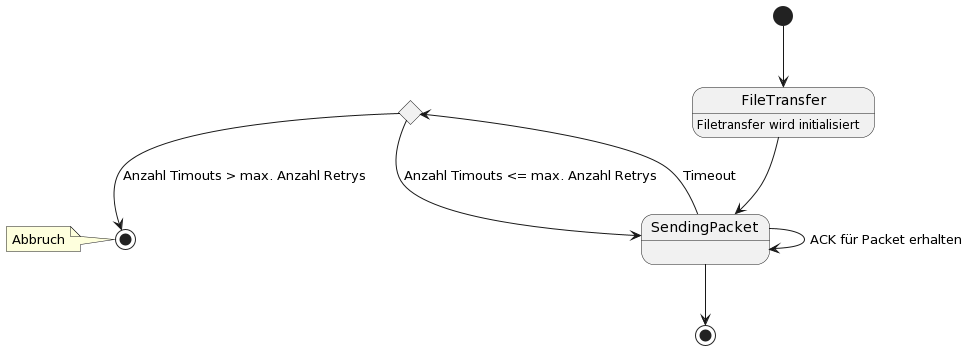
\includegraphics{client.jpg}
    \subsection{Server}
    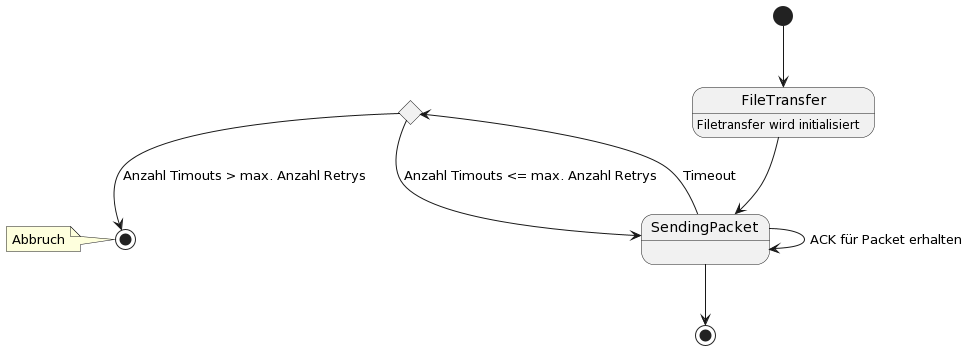
\includegraphics{client.jpg}

\end{document}